\begin{frame}{Number-like images}
  \begin{block}{Short numbers}
    \begin{itemize}
      \item PIN.
      \item Dates. 
    \end{itemize}
  \end{block}
\end{frame}

\begin{frame}{Number-like images}
  \begin{block}{Number images}
    \begin{center}
      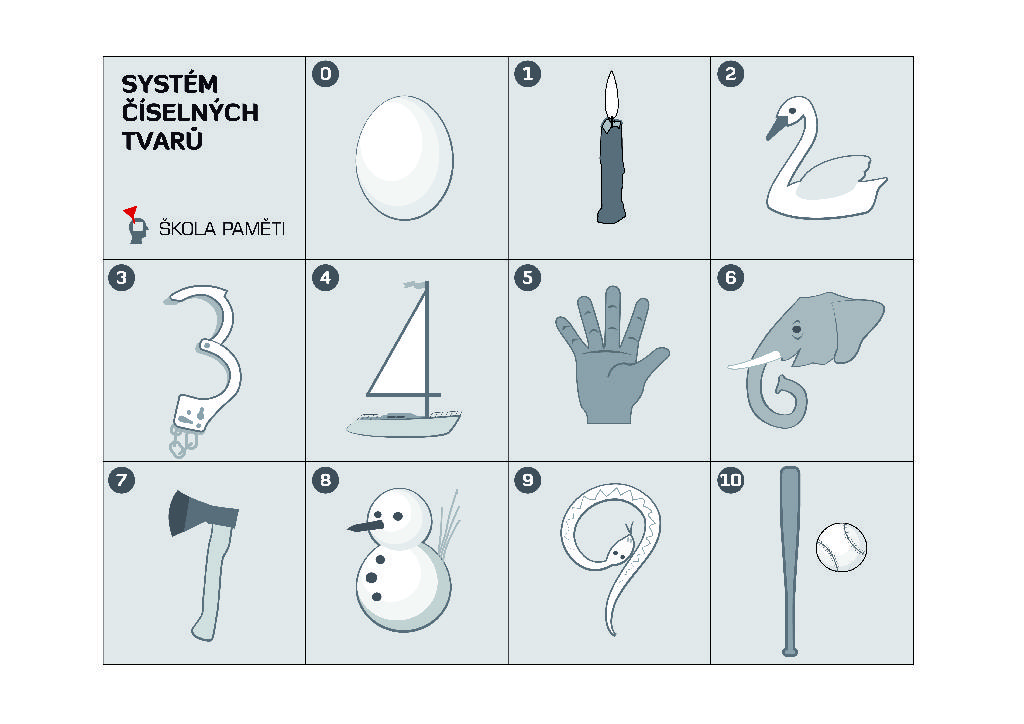
\includegraphics[height=6cm]{img/numbers.jpg}
    \end{center}
  \end{block}
\end{frame}

\begin{frame}{Number-like images}
  \begin{center}
    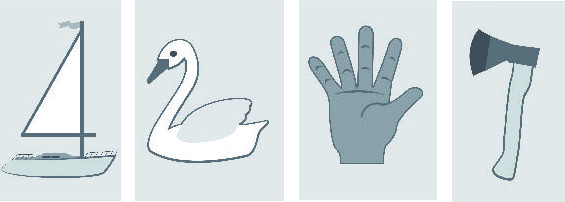
\includegraphics[height=3cm]{img/pin.jpg}
  \end{center}
  \begin{block}{PIN 4257}
    \begin{itemize}
      \item I decided to go for a sail with my YACHT. 
      \item Suddenly, I spotted a SWAN. 
      \item What a surprise! She started to shout at me. STOP, don't move. 
      \item OK, I was hungry anyway, so let's take an AXE and make dinner. 
    \end{itemize}
  \end{block}
\end{frame}

\begin{frame}{Master system}
  \begin{block}{Long numbers or sets}
    \begin{itemize}
      \item Letters represent numbers. 
      \item Words represent groups of numbers (usually of 2 or three).
    \end{itemize}
  \end{block}
\end{frame}

\begin{frame}{Master system}
  \begin{block}{First 10 digits}
    \begin{itemize}
      \item Nula $=>$ N 
      \item Jedna $=>$ J
      \item Dva $=>$ D
      \item Tri $=>$ T
      \item Ctyri $=>$ C
      \item Pet $=>$ P
      \item Sest $=>$ S
      \item sedM $=>$ M
      \item osm [neKonecno] $=>$ K
      \item deVet $=>$ V
    \end{itemize}
  \end{block}
\end{frame}

\begin{frame}{Master system}
  \begin{block}{$\pi$ = 3.14159265358}
    \begin{itemize}
      \item 31 = TJ = To Je
      \item 41 = CJ = CaJ
      \item 59 = PV = PraVil
      \item 26 = DS = DaS
      \item 53 = PT = ProTo
      \item 58 = PV = PoKracujeme
    \end{itemize}
  \end{block}
\end{frame}

\begin{frame}{Master system}
  \begin{block}{First 10 digits}
    \begin{itemize}
      \item Zero $=>$ Z
      \item oNe $=>$ N
      \item Two $=>$ T
      \item tHree $=>$ H
      \item Four $=>$ F
      \item fiVe $=>$ V
      \item Six $=>$ S
      \item seveN $=>$ N
      \item eiGht $=>$ G
      \item nine [naJn] $=>$ J 
    \end{itemize}
  \end{block}
\end{frame}

\begin{frame}{Master system}
  \begin{block}{$\pi$ = 3.14159265359}
    \begin{itemize}
      \item 31 = TZ (tizzy)
      \item 41 = HN (honey)
      \item 59 = VJ (viable) [vajabl]
      \item 26 = TS (task)
      \item 53 = VH (vehicle)
      \item 59 = VJ (via) [vaja]
    \end{itemize}
  \end{block}
\end{frame}

\begin{frame}{Calendar}
  \begin{block}{Which day is on...?}
    \begin{itemize}
      \item I can remember all week days in 2016. 
      \item Can you do that too? Yes, you can!
      \item 1 8 15 22 29
    \end{itemize}
  \end{block}
\end{frame}

\begin{frame}{Calendar}
  \begin{block}{Q1}
    \begin{itemize}
      \item Janury, Friday, I was so FRIGHTENED before my journey.
      \item February, Monday, I MOVED to my new apartment in the NL. 
      \item March, Tuesday, I started to TALK in dutch. 
    \end{itemize}
  \end{block}
\end{frame}

\begin{frame}{Calendar}
  \begin{block}{Q2}
    \begin{itemize}
      \item April, Friday, I made first FRIENDS in Arnhem. 
      \item May, Sunday, The SUN is hotter and hotter.
      \item June, Wednesday, I can't WAIT to see my family/friends again.
    \end{itemize}
  \end{block}
\end{frame}

\begin{frame}{Calendar}
  \begin{block}{Q3}
    \begin{itemize}
      \item July, Friday, I am going to be FREE from work for two weeks. 
      \item August, Monday, I am out of MONEY after vacations. 
      \item September, Thursday, I decided to THINK more deeply about things.
    \end{itemize}
  \end{block}
\end{frame}

\begin{frame}{Calendar}
  \begin{block}{Q4}
    \begin{itemize}
      \item October, Saturday, I am SATISFIED with my choice from previous month.
      \item November, Tuesday, I want a TURTLE as a Christmas present.
      \item December, Thursday, Santa is a THIEF, he stole us milk and all cookies from under the Christmas tree. 
    \end{itemize}
  \end{block}
\end{frame}

\begin{frame}{PAO system}
  \begin{block}{Principles}
    \begin{itemize}
      \item 0-9 ~ A-I or alternative mapping (e. g. based on fonetics). 
      \item List of \(famous\) people.
      \item 00-99: person-action-object.
    \end{itemize}
  \end{block}
  \begin{block}{Sample}
    \begin{itemize}
      \item 15: Albert Einstein | writing | blackboard. 
      \item 33: Charlie Chaplin | swinging | cane.
      \item 22: Bjorn Borg | playing | tennis.
      \item \dots
    \end{itemize}
  \end{block}
\end{frame}

\begin{frame}{PAO system}
  \begin{block}{Sample}
    \begin{itemize}
      \item 15: Albert Einstein | writing | blackboard. 
      \item 33: Charlie Chaplin | swinging | cane.
      \item 22: Bjorn Borg | playing | tennis.
      \item \dots
    \end{itemize}
  \end{block}
  \begin{block}{Example}
    \begin{itemize}
      \item 221533:  22-15-33. 
      \item Bjorn Borg -- writing -- (with) cane. 
    \end{itemize}
  \end{block}
\end{frame}
